\chapter{The Prior}

\vspace{1em}
\hfill
\begin{minipage}[c]{0.55\textwidth}
\raggedleft
\small\itshape
The universal a priori probability is a probability measure on the set of all possible sequences of symbols.\\[0.5em]
\upshape\footnotesize Ray Solomonoff, \textit{A Formal Theory of Inductive Inference} (1964)
\end{minipage}%
\hspace{0.5em}
\begin{minipage}[c]{0.12\textwidth}
% \includegraphics[width=\textwidth]{figures/ch04_prior.png}
\end{minipage}
\vspace{1.5em}

\noindent Bayes requires a prior. In the classical treatment, the prior is a matter of taste, of prior knowledge, or of guess. This chapter is the page where it stops being.

\section*{What kind of measure?}

The Library is the set of all possible structures, generated by descending the tree of all strings. You want a probability distribution on this Library: a way of weighting each string, and each program built from strings, so that the total weight is finite and the weights agree with the structure of the Library.

The natural first attempt is uniform. Every string of length $n$ gets weight $2^{-n}$. Two strings of length $1$ each get $1/2$; four of length $2$ each get $1/4$. The total weight at each level is exactly $1$.

The sum over all levels diverges. There are infinitely many levels.

A uniform distribution is impossible on the full Library. You cannot put equal weight on every string when there are infinitely many strings, even when you let the per-string weight shrink with length.

You have to weight shorter strings more.

\section*{Prefix-free codes}

The next attempt: weight each string $s$ by $2^{-|s|}$, where $|s|$ is its length. Length-$1$ strings each get $1/2$; length-$2$ strings each get $1/4$; and so on.

This also diverges. There are two strings of length $1$, contributing $2 \times 1/2 = 1$. Four strings of length $2$, contributing $4 \times 1/4 = 1$. And so on. The total is $1 + 1 + 1 + \dots$, unbounded.

The fix is to use only a \emph{prefix-free} subset of the strings.

A set of strings is prefix-free if no string in the set is a prefix of another. The set $\{0, 10, 11\}$ is prefix-free. The set $\{0, 01, 11\}$ is not: $0$ is a prefix of $01$.

In the tree of all strings (Figure~\ref{fig:enumeration-tree} from Chapter 2), a prefix-free set corresponds to a collection of nodes whose subtrees are disjoint. Whenever you select a node as a codeword, you cannot also select any of its descendants. The codeword ``claims'' its entire subtree. Figure~\ref{fig:prefix-free-tree} shows an example.

\begin{figure}[h]
\centering
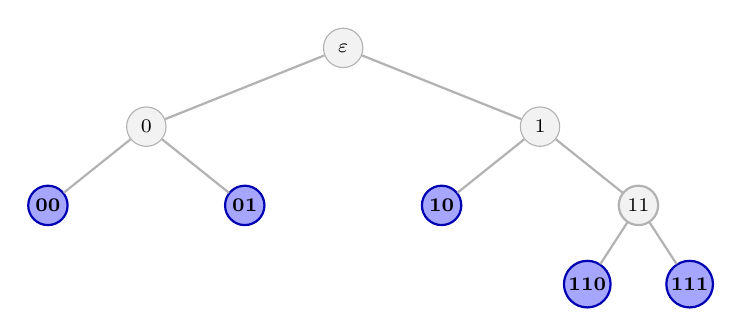
\begin{tikzpicture}[
  level distance=1cm,
  level 1/.style={sibling distance=5cm},
  level 2/.style={sibling distance=2.5cm},
  level 3/.style={sibling distance=1.3cm},
  edge from parent/.style={draw, thick, gray!60}
]
  \node[circle, draw=gray!60, fill=gray!10, inner sep=1pt, minimum size=5mm, font=\scriptsize] {$\varepsilon$}
    child {node[circle, draw=gray!60, fill=gray!10, inner sep=1pt, minimum size=5mm, font=\scriptsize] {0}
      child {node[circle, draw=blue!70!black, fill=blue!35, inner sep=1pt, minimum size=5mm, font=\scriptsize\bfseries] {00}}
      child {node[circle, draw=blue!70!black, fill=blue!35, inner sep=1pt, minimum size=5mm, font=\scriptsize\bfseries] {01}}
    }
    child {node[circle, draw=gray!60, fill=gray!10, inner sep=1pt, minimum size=5mm, font=\scriptsize] {1}
      child {node[circle, draw=blue!70!black, fill=blue!35, inner sep=1pt, minimum size=5mm, font=\scriptsize\bfseries] {10}}
      child {node[circle, draw=gray!60, fill=gray!10, inner sep=1pt, minimum size=5mm, font=\scriptsize] {11}
        child {node[circle, draw=blue!70!black, fill=blue!35, inner sep=1pt, minimum size=5mm, font=\scriptsize\bfseries] {110}}
        child {node[circle, draw=blue!70!black, fill=blue!35, inner sep=1pt, minimum size=5mm, font=\scriptsize\bfseries] {111}}
      }
    };
\end{tikzpicture}
\caption{A prefix-free code as a set of disjoint subtrees. The codewords (filled in blue) are $\{00, 01, 10, 110, 111\}$. Each codeword sits at a node whose entire subtree is ``claimed.'' No codeword is the prefix of another, so the claimed subtrees do not overlap. In this case the codewords also cover the tree: every infinite path passes through exactly one of them.}
\label{fig:prefix-free-tree}
\end{figure}

\section*{Kraft's inequality}

For any prefix-free code with codeword lengths $\ell_1, \ell_2, \ldots$,

$$\sum_i 2^{-\ell_i} \leq 1.$$

This is Kraft's inequality, proved in 1949. The proof is one paragraph.

Consider the unit interval $[0, 1]$. Each codeword $s$ of length $|s|$ corresponds to a sub-interval of width $2^{-|s|}$: the set of real numbers in $[0,1)$ whose binary expansion begins with $s$. The codeword $0$ corresponds to $[0, 1/2)$. The codeword $11$ corresponds to $[3/4, 1)$. The codeword $001$ corresponds to $[1/8, 1/4)$.

If the code is prefix-free, no two of these sub-intervals overlap, because no codeword is a prefix of another. The total width of the sub-intervals is at most $1$, the width of the whole unit interval.

That is Kraft. Prefix-free codes correspond to non-overlapping sub-intervals; non-overlapping sub-intervals fit inside the unit interval; the total widths sum to at most $1$. Figure~\ref{fig:kraft-interval} shows the tiling for the same code.

\begin{figure}[h]
\centering
\begin{tikzpicture}[scale=0.85]
  % Unit interval as a rectangle
  \draw[thick] (0,0) rectangle (12,0.9);
  % Subdivisions for code {00, 01, 10, 110, 111}
  \draw[thick] (3,0) -- (3,0.9);
  \draw[thick] (6,0) -- (6,0.9);
  \draw[thick] (9,0) -- (9,0.9);
  \draw[thick] (10.5,0) -- (10.5,0.9);
  % Codeword labels
  \node[font=\small] at (1.5, 0.45) {$00$};
  \node[font=\small] at (4.5, 0.45) {$01$};
  \node[font=\small] at (7.5, 0.45) {$10$};
  \node[font=\small] at (9.75, 0.45) {$110$};
  \node[font=\small] at (11.25, 0.45) {$111$};
  % Width annotations above
  \draw[<->, thick] (0, 1.2) -- (3, 1.2);
  \node[anchor=south, font=\scriptsize] at (1.5, 1.2) {$2^{-2}$};
  \draw[<->, thick] (9, 1.2) -- (10.5, 1.2);
  \node[anchor=south, font=\scriptsize] at (9.75, 1.2) {$2^{-3}$};
  % Total
  \node[anchor=north, font=\small] at (6, -0.2) {total width $= \tfrac{1}{4} + \tfrac{1}{4} + \tfrac{1}{4} + \tfrac{1}{8} + \tfrac{1}{8} = 1$};
\end{tikzpicture}
\caption{Kraft's inequality as unit-interval tiling. The same prefix-free code $\{00, 01, 10, 110, 111\}$ from Figure~\ref{fig:prefix-free-tree} partitions the unit interval. Each codeword $s$ owns a sub-interval of width $2^{-|s|}$. Because the code is prefix-free, the sub-intervals do not overlap. Their total width is at most $1$. In this case the code is complete and the total is exactly $1$.}
\label{fig:kraft-interval}
\end{figure}

\section*{Length becomes probability}

Kraft is a fact about prefix-free codes. It becomes a probability distribution by a renaming.

For any prefix-free code, define

$$P(s) = 2^{-|s|}$$

for each codeword $s$. The sum is $\sum_s P(s) = \sum_s 2^{-|s|} \leq 1$ by Kraft. If the sum is less than $1$, treat the missing mass as a residual ``unused'' probability. If the sum equals $1$, the codewords cover everything.

The function $P$ is a probability distribution on the codewords. Shorter codewords have higher probability; longer codewords have lower probability. This is no longer an aesthetic preference. It is what the geometry of prefix-free codes makes available.

What the geometry makes \emph{impossible}: a probability distribution that does not favor shorter codewords. The structure of the tree, the constraint of prefix-freedom, and the bookkeeping of probability together force the simpler-is-more-likely property. You cannot put more weight on long codewords than on short ones, on average, and still satisfy Kraft.

The simplicity bias is not a heuristic. It is the only probability the Library admits.

\section*{The universal prior}

Now extend from codewords to programs. Programs are strings; they differ from arbitrary strings only in that they have a runtime behavior on a universal computer.

Let $U$ be a universal Turing machine whose input set is prefix-free: every halting input is a complete program, not the prefix of a longer one. Such machines exist and are standard.\footnote{Any universal machine can be made prefix-free by including the program's length as a header, or by self-delimiting techniques developed by Chaitin and Levin in the 1970s. The technical details do not affect the argument.} For each program $p$ that produces the string $x$ as the start of its output (Figure~\ref{fig:prefix}), give it weight $2^{-|p|}$. Sum over all such programs:

$$M(x) = \sum_{p \,:\, U(p) = x*} 2^{-|p|}.$$

\begin{figure}[h]
\centering
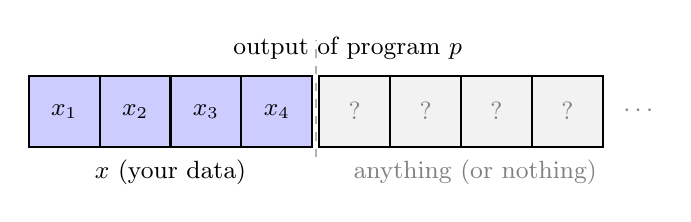
\begin{tikzpicture}[scale=0.9]
  % Prefix x: filled blue boxes
  \foreach \i/\lbl in {0/{$x_1$}, 1/{$x_2$}, 2/{$x_3$}, 3/{$x_4$}} {
    \draw[thick, fill=blue!20] (\i, 0) rectangle ({\i+1}, 1);
    \node[font=\small] at ({\i+0.5}, 0.5) {\lbl};
  }

  % Dashed separator
  \draw[thick, dashed, gray!60] (4.05, -0.15) -- (4.05, 1.5);

  % Continuation: gray "?" boxes
  \foreach \i in {0, 1, 2, 3} {
    \draw[thick, fill=gray!10] ({\i+4.1}, 0) rectangle ({\i+5.1}, 1);
    \node[font=\small, gray] at ({\i+4.6}, 0.5) {$?$};
  }
  \node[font=\small, gray] at (8.6, 0.5) {$\cdots$};

  % Labels below
  \node[anchor=north, font=\small] at (2, -0.05) {$x$ (your data)};
  \node[anchor=north, font=\small, gray] at (6.3, -0.05) {anything (or nothing)};

  % Label above
  \node[anchor=south, font=\small] at (4.5, 1.1) {output of program $p$};
\end{tikzpicture}
\caption{The notation $U(p) = x*$ means program $p$ outputs $x$ as the beginning of its run, followed by any continuation (or none). $M(x)$ sums the weights of all programs whose outputs begin with $x$.}
\label{fig:prefix}
\end{figure}

This is the \emph{universal prior} on output strings $x$. It is a probability distribution on the Library of computable structures.\footnote{Strictly, $M$ is a semi-measure: the sum over all $x$ may be less than $1$, because some programs do not halt. The missing mass is the probability that a randomly chosen program never produces an output. The detail does not affect the chapter's argument.} Figure~\ref{fig:universal-prior} shows $M(x)$ as a cumulative sum over the programs that produce $x$, ordered by length.

\begin{figure}[h]
\centering
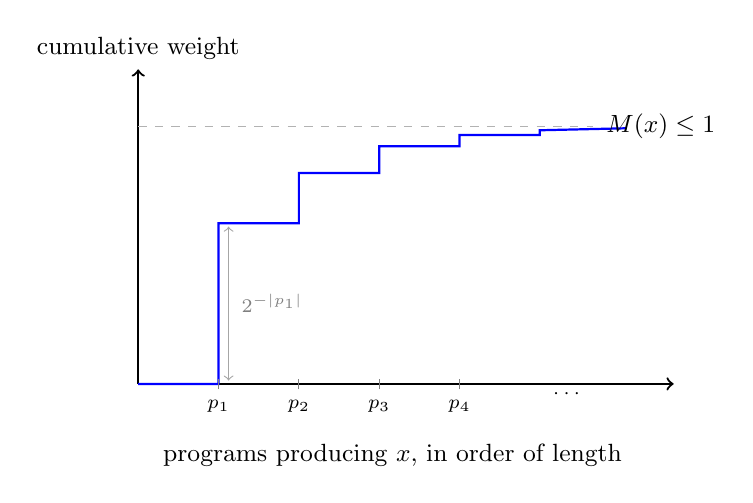
\begin{tikzpicture}[scale=0.85]
  % Axes
  \draw[->, thick] (0, 0) -- (8, 0);
  \draw[->, thick] (0, 0) -- (0, 4.7) node[above, font=\small] {cumulative weight};

  % Asymptote
  \draw[dashed, gray!60] (0, 3.85) -- (6.8, 3.85);

  % Step function (decreasing increments)
  \draw[thick, blue, line cap=square]
    (0, 0) -- (1.2, 0) -- (1.2, 2.4)
    -- (2.4, 2.4) -- (2.4, 3.15)
    -- (3.6, 3.15) -- (3.6, 3.55)
    -- (4.8, 3.55) -- (4.8, 3.72)
    -- (6, 3.72) -- (6, 3.79)
    -- (7.3, 3.82);

  % Tick marks and program labels
  \foreach \x/\p in {1.2/{$p_1$}, 2.4/{$p_2$}, 3.6/{$p_3$}, 4.8/{$p_4$}} {
    \draw[gray] (\x, -0.08) -- (\x, 0.08);
    \node[anchor=north, font=\scriptsize] at (\x, -0.1) {\p};
  }
  \node[font=\scriptsize] at (6.4, -0.15) {$\cdots$};

  % Asymptote label (placed at end of asymptote, inside the plot area)
  \node[anchor=west, font=\small] at (6.85, 3.85) {$M(x) \leq 1$};

  % First step height annotation (inside plot, right of the first step)
  \draw[<->, gray!70, thin] (1.35, 0.05) -- (1.35, 2.35);
  \node[anchor=west, font=\scriptsize, gray] at (1.4, 1.2) {$2^{-|p_1|}$};

  % X-axis caption (below, centered)
  \node[anchor=north, font=\small] at (3.8, -0.75) {programs producing $x$, in order of length};
\end{tikzpicture}
\caption{The universal prior $M(x)$ as a cumulative step function. Each program $p$ that produces $x$ contributes $2^{-|p|}$ to the cumulative sum. The shortest programs come first and contribute the largest steps. The steps shrink geometrically. The sum converges to $M(x)$, which is bounded by $1$. Most of the mass sits on a few short programs; the long tail is the contribution of the longer ways to produce the same output.}
\label{fig:universal-prior}
\end{figure}

What $M$ does, in three sentences. It assigns higher probability to strings that have shorter programs producing them. It assigns positive probability to every string that any program produces. The probability of $x$ is dominated by the contribution of the shortest program for $x$: the rest is in the tail.

What $M$ is doing, philosophically. It is putting probability weight on the Library according to how much code it takes to point to each book. Books with short addresses are common. Books with long addresses are rare. The address itself is the structure of the prior.

\section*{Where this leaves you}

Bayes needed a prior. The Library, via Kraft and prefix-free codes, hands you one.

The prior is no longer subjective. It is no longer a matter of taste. It is the unique distribution that arises from putting probability weight on a prefix-free code over a universal computer, with shorter codes getting more weight by the geometry of the tree.

When you condition on data, when you ask about hypotheses, when you ask \emph{where am I in the Library}, the prior is what answers.

But $M$ is only one prior. A reasonable agent could write down a different one. Why should this one be privileged?

The answer is the next chapter. It is a theorem. The universal prior catches up to any other prior, asymptotically, no matter what the world is doing.

That is the optimality.
